\section{Introduction}

ppcemu is a user-level PowerPC (MPC7447A) simulator with Linux System Call Translation capabilities. Computations on IEEE 754 floating point numbers are emulated using simfloat. Altivec instructions are currently decoded but not implemented. The simulator can run an application compiled for Linux PowerPC, but it can’t run a real operating system as ppcemu-system can do. Software running on the simulated hardware can be debugged by connecting a GDB client to the simulator through the GDB serial remote protocol. The GDB client can be either the standard text based client (i.e. command gdb), a graphical front-end to GDB (e.g. ddd), or even Eclipse CDT.

\begin{figure}[!h]
	\begin{center}
		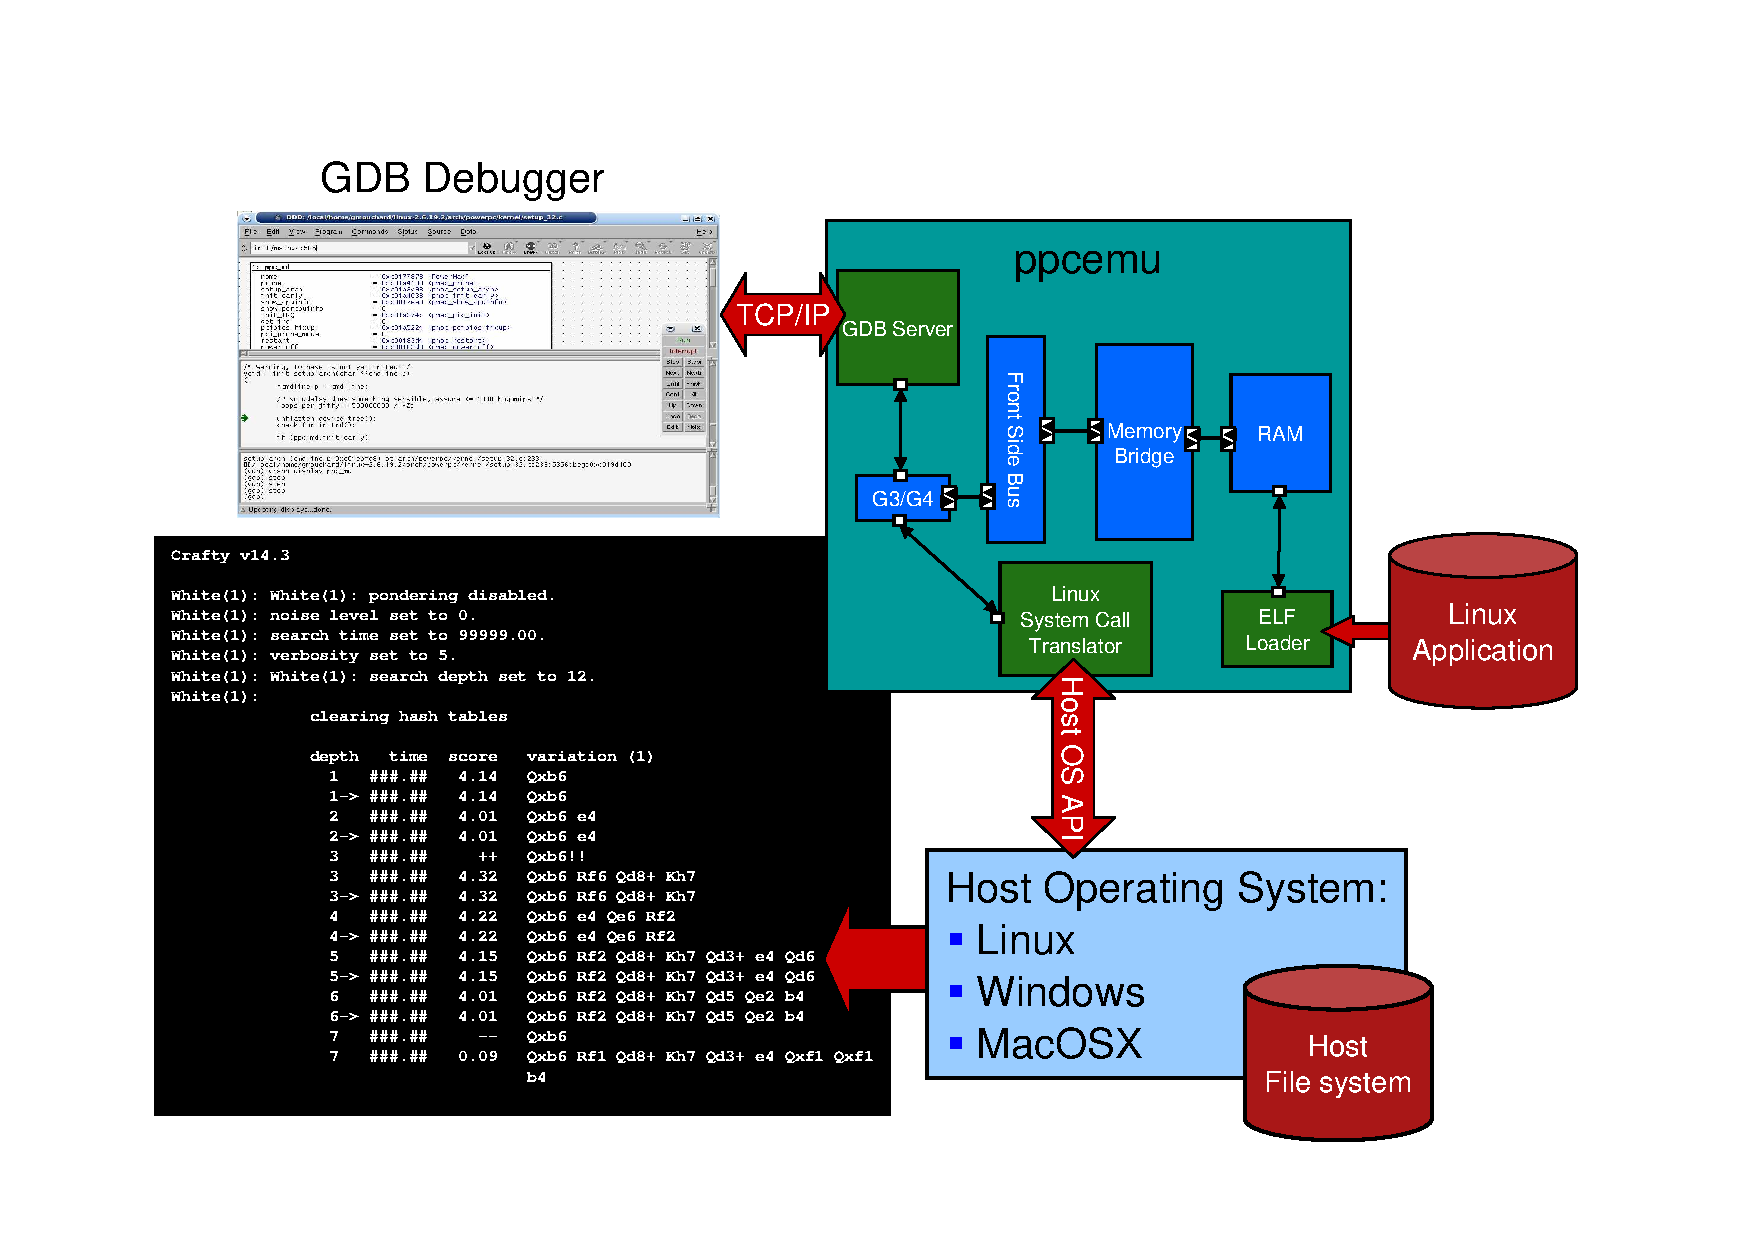
\includegraphics[width=\textwidth]{ppcemu/fig_ppcemu.pdf}
	\end{center}
	\caption{ppcemu simplified schematic.}
	\label{fig:ppcemu_system}
\end{figure}

\section{Simulated configuration}

The simulator is composed of the following modules:
\begin{itemize}\addtolength{\itemsep}{-0.40\baselineskip}
\item PowerPC CPU configured as an MPC7447A
\item snooping bus (front side bus)
\item Snooping bus to memory bridge
\item memory
\end{itemize}

The simulator uses the following services:
\begin{itemize}\addtolength{\itemsep}{-0.40\baselineskip}
\item ELF loader
\item GDB Server
\item Inline debugger
\item SystemC Time
\item Host Time
\item Power Estimators (for ITLB, DTLB, IL1, DL1 and L2)
\end{itemize}

\section{Using the simulator}

Usage: \texttt{ppcemu [<options>] <program> [program arguments]}

'program' is statically linked ELF32 PowerPC Linux program

Options:

\begin{itemize}

\item Starting the inline debugger

\texttt{--inline-debugger}
\texttt{-d}

\item Starting a GDB server

\texttt{--gdb-server <TCP port>}
\texttt{-g <TCP port>}

The GDB server will wait for a GDB client connection on the specified TCP port.

\item Defining the architecture description to be used by the GDB server

\texttt{--gdb-server-arch-file <arch file>}
\texttt{-a  <arch file>}

\item Defining the number of instructions to simulate before exiting

\texttt{-i <count>}
\texttt{--max:inst <count>}

\item Enabling power estimation for ITLB, DTLB, IL1, DL1, and L2

\texttt{-p}
\texttt{--power}

\item Redirecting the logger output into a file

\texttt{-l <file>}
\texttt{--logger:file <file>}

\item Enabling compression (gzip format) of the logger output

\texttt{-z}
\texttt{--logger:zip}

\item Redirecting the logger output to the standard error output

\texttt{-e}
\texttt{--logger:error}

\item Redirecting the logger output to the standard output

\texttt{-o}
\texttt{--logger:out}

\item Displaying the integrated help

\texttt{--help}
\texttt{-h}

\end{itemize}